\label{delta_dist_resultats}

\subsection{Estimation des performances lors de l'entraînement}

\label{delta_dist_estim_perf}

Lors de l'entraînement d'un modèle, la sortie texte de tensorflow et la sortie graphique de tensorboard (\ref{dist_rel_quadri}) permettent d'avoir une estimation de la valeur de la fonction de coût (\ref{delta_dist_eval_cout}) sur des données qui lui sont inconnues. Cela permet d'avoir une idée de la performance relative des modèles, sans faire d'analyse détaillée comme dans la section suivante. Tous les modèles décrits dans ce chapitre (en dehors des modèles les moins performants de la recherche par quadrillage) ont des performances très similaires pendant l'entraînement. Les modèles travaillant sur des données ayant un bruit de RMSE  2,8 pm (resp. 17.2 pm) effectuent des prédictions de RMSE 1,8 pm (resp. 10,7 pm). Dans les deux cas, cela revient à réduire l'erreur à environ 63\% de sa valeur initiale, et donc à prédire 37\% du bruit. Il s'agit d'un gain non négligeable, mais nous allons montrer dans la sous-partie suivante qu'il n'est pas réellement utilisable pour optimiser la géométrie des molécules.

\subsection{Analyse détaillée d'un modèle}

\par Nous allons ici analyser les prédictions du modèle \emph{DELTA\_DIST\_+H\_05}. Tous les modèles ayant des performances similaires, nous supposons que l'analyse de leurs résultats est similaire à celle que l'on développe ici.

\par Le modèle ayant une sortie composée de multiples valeurs, nous allons décomposer ses prédictions afin de pouvoir les analyser. Ce que l'on va nommer par la suite prédictions est l'ensemble des composantes de tous les vecteurs de sortie du modèle sur le jeu de test après l'application d'un masque ne sélectionnant que les composantes de sortie correspondant à des atomes définis en entrée (\ref{delta_dist_homogen}). De même, ce que l'on nomme cibles est l'ensemble des valeurs attendues en sortie sur tous les exemples du jeu de test après sélection des valeurs correspondant à des atome définis, et le vecteur erreurs est alors la valeur absolue de la différence entre ces deux vecteurs.

\subsubsection{Analyse statistique}

\par Dans un premier temps, nous allons effectuer une analyse statistique des valeurs présentes dans les vecteurs cibles (tableau \ref{t_stats_delta_dist_cibles}), prédictions (tableau \ref{t_stats_delta_dist_preds}) et erreurs (tableau \ref{t_stats_delta_dist_errs}). \\


\begin{table}
	\centering
	\begin{tabular}{|l|r|}
		\hline
		Moyenne & -0,8216 \\ \hline
		Médiane & -0,8198 \\ \hline
		Écart-type & 17,3062 \\ \hline
		Minimum & -94,7950 \\ \hline
		Maximum & 97,2401 \\ \hline
	\end{tabular}
	
	\caption{Analyse statistique des valeurs cibles (en pm)}
	\label{t_stats_delta_dist_cibles}
\end{table}

\par Les cibles correspondent au déplacement des atomes de la molécule par le bruit relativement à quatre points fixes du repère (\ref{repr_mat_pts_fixes}). Le bruit étant gaussien, la moyenne et la médiane sont comme attendu très proches. L'écart-type des déplacements est très proche de la valeur donnée comme paramètre lors de l'introduction du bruit (\ref{delta_dist_prep_bruit}), ce qui est également prévisible. Le fait d'ajouter le bruit sur les coordonnées plutôt que sur les distances a cependant déplacé le déplacement moyen de zéro vers une valeur légèrement négative, c'est à dire que les atomes ont en moyenne été plus rapprochés de l'origine du repère qu'éloignés.\\


\begin{table}
	\centering
	\begin{tabular}{|l|r|}
		\hline
		Moyenne & -0,2328 \\ \hline
		Médiane & -0,1346 \\ \hline
		Écart-type & 10,4515 \\ \hline
		Minimum & -9,5675 \\ \hline
		Maximum & 1,2347 \\ \hline
	\end{tabular}
	
	\caption{Analyse statistique des prédictions (en pm)}
	\label{t_stats_delta_dist_preds}
\end{table}

\par La moyenne et la médiane des prédictions étant décalées, elles ne suivent pas une distribution gaussienne comme attendu. L'intervalle des valeurs prédites n'est pas centré sur zéro mais est nettement déplacé vers les valeurs négatives. Cela s'explique par le centrage des cibles sur une valeur légèrement négative.
L'écart-type n'étant pas comparable avec l'écart-type des valeurs cibles car la distribution n'est pas gaussienne, il est difficile d'estimer la dispersion des prédictions. Elles semblent toutefois très proches de zéro, comparativement aux valeurs attendues. En effet, les prédictions s'étendent entre -9,6 et 1,2, alors qu'on souhaiterait qu'elles s'étendent entre -94,8 et 97,2 dans les cas extrêmes, et qu'elles soient comprises entre -30,0 et 30,0 dans le cas général (\ref{delta_dist_prep_bruit}). Le modèle  n'arrive donc pas à suffisamment déplacer les atomes pour obtenir les géométries convergées.\\


\begin{figure}
	\centering
	\begin{tabular}{|l|r|}
		\hline
		Moyenne & 13,8335 \\ \hline
		Médiane & 11,6937 \\ \hline
		Écart-type & 10,4515 \\ \hline
		Minimum & 0,0000 \\ \hline
		Maximum & 97.7970 \\ \hline
	\end{tabular}
	
	\caption{Analyse statistique des erreurs absolues (en pm)}
	\label{t_stats_delta_dist_errs}

\end{figure}

\par On souhaiterait que les erreurs soient de l'ordre de 1 pm, alors qu'elles sont en moyenne de 13,9 pm. Cette erreur moyenne importante est prévisible puisque les prédictions sont dans un intervalle d'amplitude environ vingt fois plus faible que l'amplitude de l'intervalle des valeurs cibles.\\

\subsubsection{Distribution de l'erreur absolue}

Afin de comprendre la façon dont les erreurs sont distribuées, nous représentons graphiquement leur représentation en fonction de leur valeur.

\begin{figure}
	\centering
	
	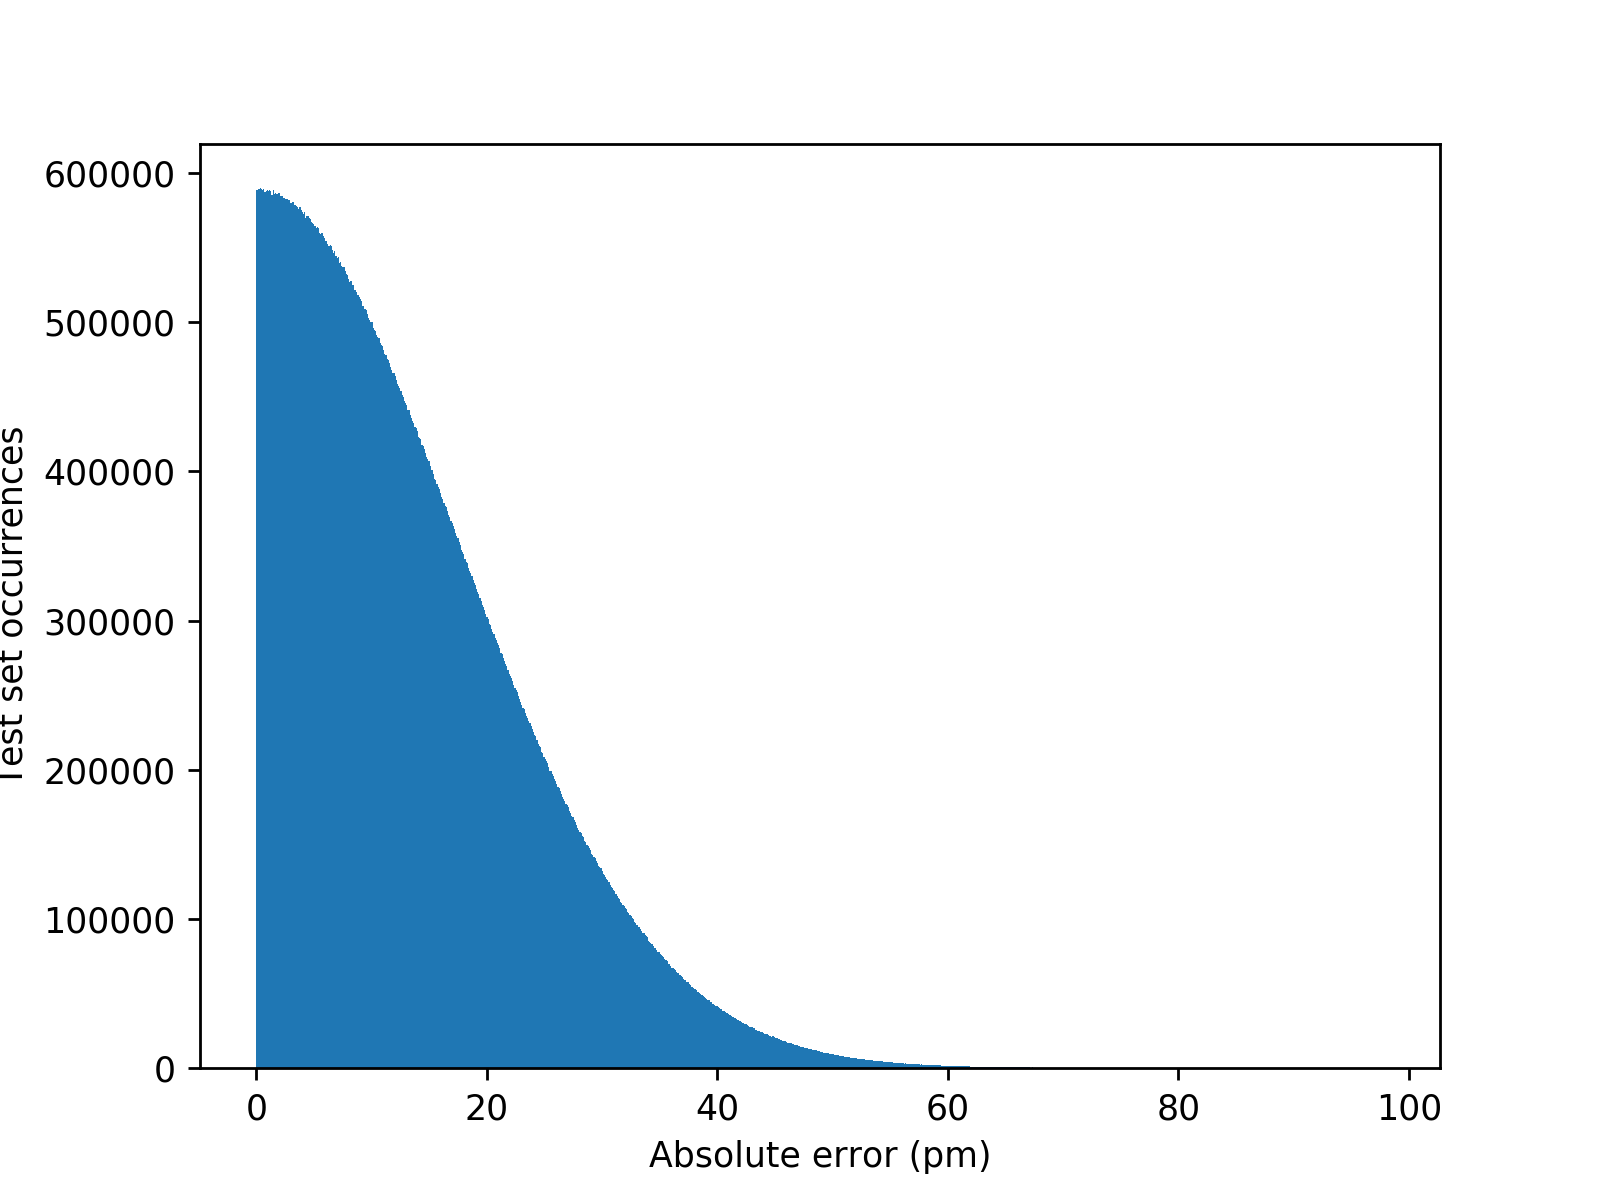
\includegraphics[scale=0.7]{../figures/DELTA_DIST_+H_05/DELTA_DIST+H_05_distrib_rmse_val.png}	
	
	\caption{Distribution des erreurs du modèle \emph{DELTA\_DIST\_+H\_05}}
	\label{fig_distrib_err_delta_dist}
\end{figure}

L'erreur (figure \ref{fig_distrib_err_delta_dist}) semble suivre une distribution gaussienne. L'erreur présentée ici étant l'erreur absolue, nous ne voyons qu'une demie courbe de Gauss. Cela montre que le bruit a été en partie « absorbé » par la prédiction, mais que sa distribution est restée semblable.

\subsubsection{Distribution de l'erreur absolue en fonction des cibles}

La représentation de la distribution de l'erreur absolue en fonction des cibles (figure \ref{fig_distrib_err_rel_delta_dist}) montre que la majorité des prédictions sont très proches de zéro, et que les autres sont proches de -9. Il s'agit probablement d'une méthode pour le modèle de minimiser « en moyenne » la fonction de coût. Les prédictions autour de -9 font probablement partie des raisons pour laquelle la fonction de coût diminue de 37\% par rapport à l'erreur introduite par le bruit.


\begin{figure}
	\centering
	
	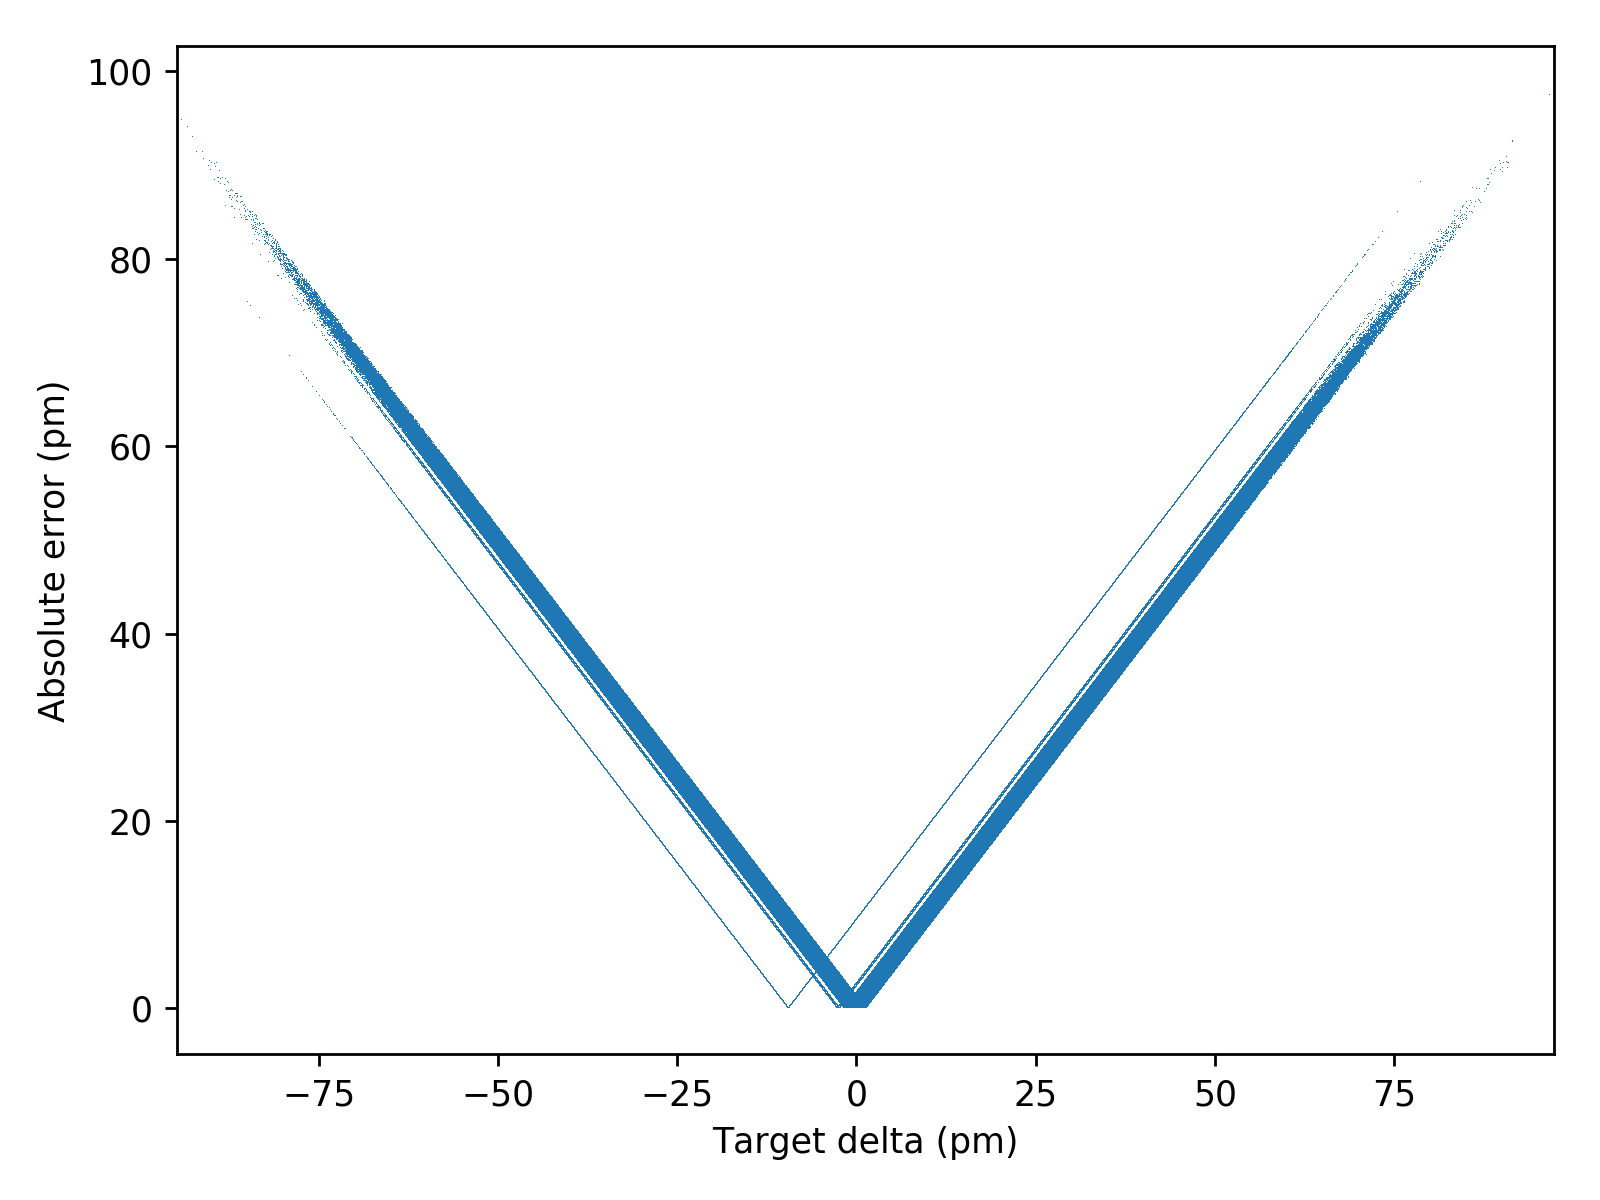
\includegraphics[scale=0.7]{../figures/DELTA_DIST_+H_05/DELTA_DIST+H_05_distrib_rmse_dist.png}	
	
	\caption{Erreur en fonction des cibles pour le modèle \emph{DELTA\_DIST\_+H\_05}}
	\label{fig_distrib_err_rel_delta_dist}

	\end{figure}



\subsubsection{Distribution des prédictions en fonctions des cibles}

\begin{figure}
	\centering
	
	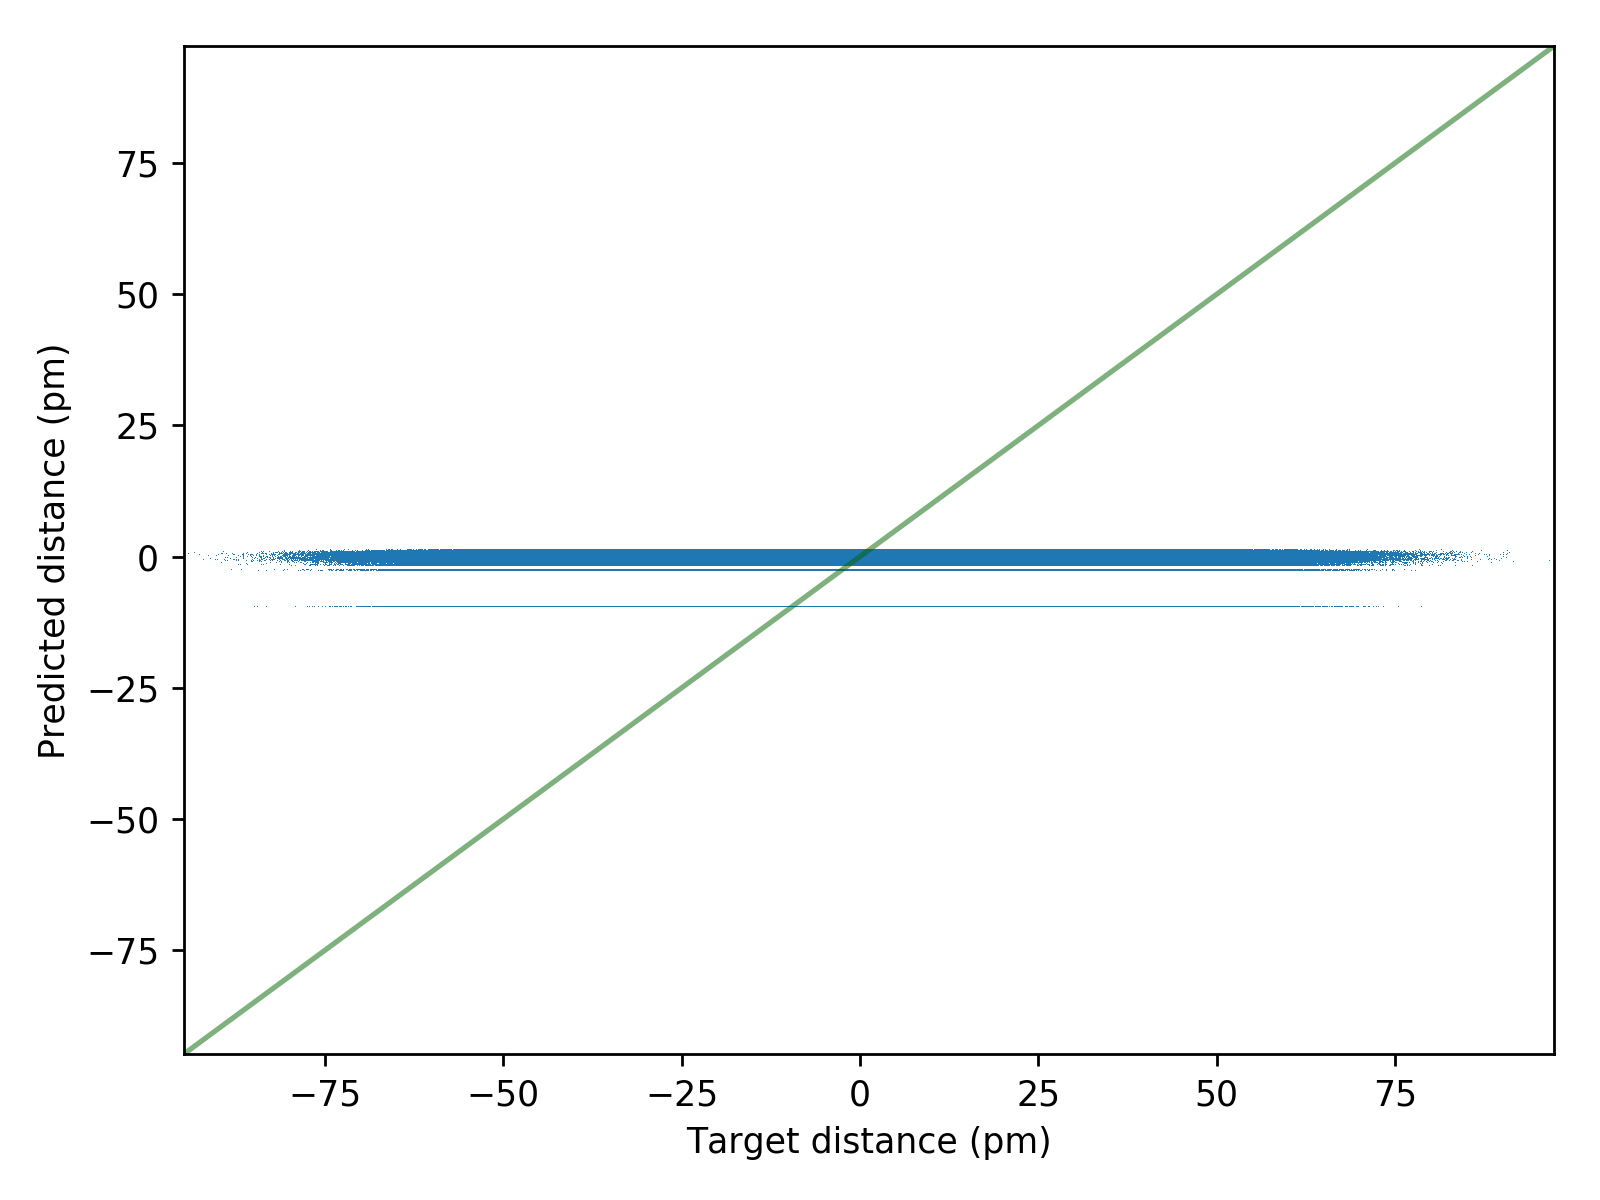
\includegraphics[scale=0.7]{../figures/DELTA_DIST_+H_05/DELTA_DIST+H_05_preds_targets.png}	
	
	\caption{Prédictions en fonction des cibles pour le modèle \emph{DELTA\_DIST\_+H\_05}}
	\label{fig_preds_targets_delta_dist}

	
\end{figure}

\par La droite tracée (figure \ref{fig_preds_targets_delta_dist}) correspond aux prédictions attendues. Les prédictions du modèle ont une intersection avec la droite limitée aux prédictions proches de zéro et de -9.

\begin{figure}	

	\centering
	
	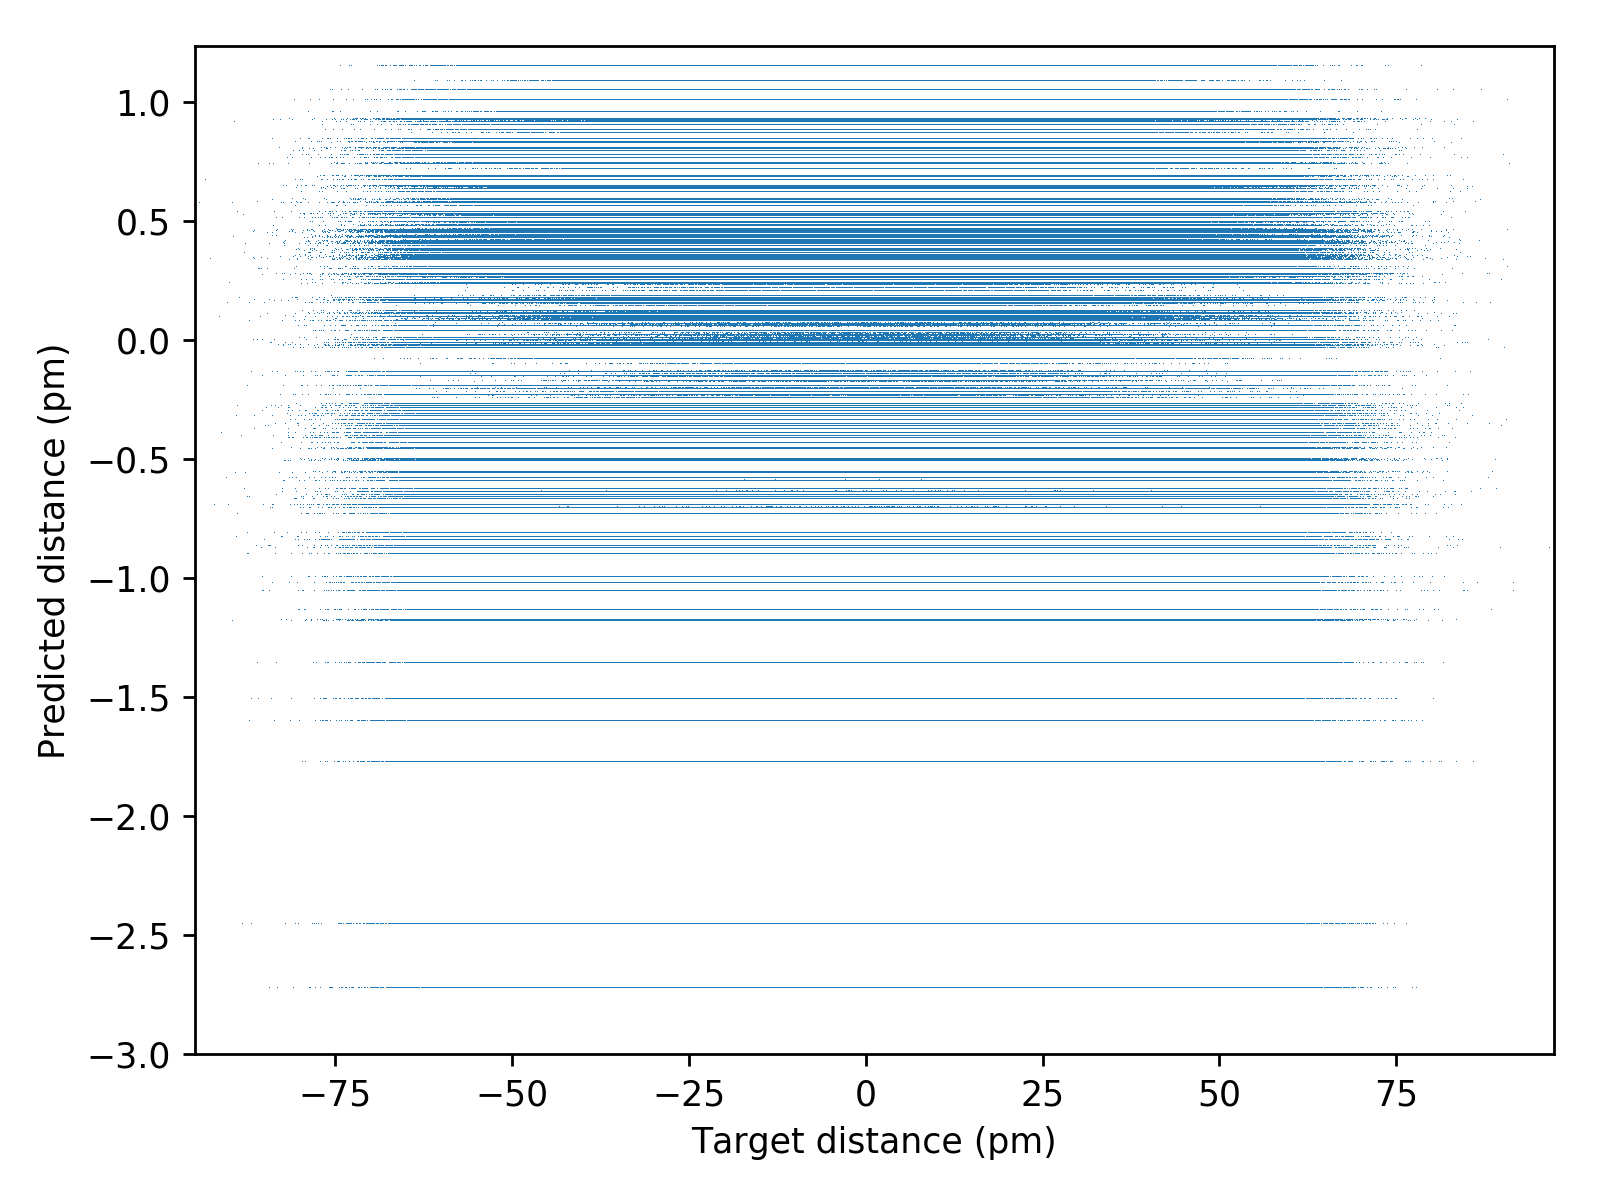
\includegraphics[scale=0.7]{../figures/DELTA_DIST_+H_05/DELTA_DIST+H_05_preds_targets_zoom.png}	
	
	\caption{Prédictions en fonction des cibles pour le modèle \emph{DELTA\_DIST\_+H\_05} (zoom)}
	\label{fig_zoom_preds_targets_delta_dist}

	
\end{figure}
\par Lorsque l'on regarde de plus près les prédictions (figure \ref{fig_zoom_preds_targets_delta_dist}), on s'aperçoit qu'elles prennent des valeurs discrètes. Cette subtilité peut en partie expliquer la capacité du modèle à prédire partiellement le bruit.

\subsection{Abandon de la méthode}
\label{delta_dist_abandon}

Le fait que le modèle effectue des prédictions constantes et l'impossibilité de produire de meilleurs résultats à l'issue de la recherche par quadrillage (\ref{delta_dist_quadri}) ont mené à l'abandon de la méthode pour prédire des géométries moléculaires convergées, au profit d'une méthode moins ambitieuse (chapitre \ref{dist_rel_chap}).\\

\par Il est démontré qu'il existe une fonction permettant d'optimiser la géométrie moléculaire, et que les réseaux de neurones sont des approximateurs universels de fonctions\cite{universal_approx}. La tâche que nous avons tenté d'accomplir avec ces modèles est donc théoriquement possible. Nous pouvons toutefois trouver quelques explications possibles à notre incapacité à entraîner un modèle suffisamment efficace. 

\par Premièrement, les modèles que nous avons entraînés sont des modèles aux architectures relativement simples, avec un nombre de neurones et de connexions limité par les capacités matérielles. Des architectures plus complexes auraient pu mener à de meilleures performances pour les mêmes données. \\
Un autre écueil pourrait être le manque de données. Même si nous travaillons sur un jeu de données contenant 3,7 millions de molécules (\ref{donnees_bases}), il s'agit peut-être d'une quantité insuffisante pour approximer correctement une fonction aussi complexe. De même, il est possible qu'il manque certains descripteurs des molécules en entrée des modèles.\\
Enfin, il est possible que le problème soit lié à notre méthodologie, et notamment au fait que l'on génère un jeu d'entraînement en ajoutant du bruit sur les données à prédire. Peut-être la tâche de prédiction est-elle impossible à réaliser à cause du caractère aléatoire et par définition imprédictible du bruit gaussien. On peut tout de même raisonnablement imaginer que si un modèle est capable de prédire une géométrie convergée, il est capable de soustraire la géométrie convergée d'une géométrie bruitée.